\documentclass[12pt]{article} %set font size and document type
\usepackage{graphicx} % Required for inserting images
\usepackage{tocloft}
\usepackage{enumitem}
\usepackage[dvipsnames]{xcolor}
\usepackage{tabularx}
\usepackage{float}
\usepackage{xcolor}

\renewcommand{\cftsecfont}{\large\bfseries}
\renewcommand{\cftsecpagefont}{\large\bfseries}

\renewcommand{\cftsubsecfont}{\normalsize}
\renewcommand{\cftsubsecpagefont}{\normalsize}

\setlength{\cftbeforesecskip}{10pt}
\setlength{\cftbeforesubsecskip}{5pt}

\usepackage[useregional]{datetime2} %allow use of \today
\usepackage[margin=1in]{geometry} % set margins
\usepackage{setspace} % allow setting of double and single spacing
\usepackage{hyperref} % creates clickable table of contents
\usepackage{adjustbox} % allows us to rotate images, tables, etc.

% \usepackage{xcolor}
\usepackage{color, colortbl}

\usepackage{listings}
\newcommand{\lsin}[1]{\lstinline[columns=fullflexible,keepspaces=true,language=Java,basicstyle=\footnotesize\ttfamily]{#1}}

\lstdefinelanguage{Java}{
  columns=fullflexible,keepspaces=true,basicstyle=\scriptsize\ttfamily,
%  basicstyle=\scriptsize\sffamily,
  numbers=left,
  xleftmargin=5.0ex,
  escapechar=@,
  sensitive=true,
  otherkeywords={},
  morekeywords=[1]{int,while,if,public,static,else,return,new,for,return,void},
  keywordstyle={[1]\bfseries\color{blue}},
  numberstyle=\tiny\color{black},
  rulecolor=\color{black},
}

% set up header and footer
\usepackage{titleps,kantlipsum}
\newpagestyle{mypage}{%
  \headrule
  \sethead{\MakeUppercase{\thesection\quad \sectiontitle}}{}{\thesubsection\quad \subsectiontitle}
  \setfoot{}{}{\em{p. \thepage}}
}
\settitlemarks{section,subsection}
\pagestyle{mypage}

\title{CS482 Sprint 3 Deliverable}
\author{Ryland, Silas, Marley, and Chase\\
Client: Dr. Hoang Bui}
\date{November 2024}

\begin{document}

\maketitle
\pagebreak
\setcounter{subsection}{0}
\tableofcontents
\newpage

\section{User Stories}
\begin{table}[htbp]
\centering
\small
\begin{tabularx}{\textwidth}{|l|l|p{1cm}|X|X|}
\hline
\textbf{ID} & \textbf{Points} & \textbf{As a [user type]} & \textbf{I want [functionality]} & \textbf{So that [value]} \\ \hline
S1 & 2 & Player & to create an account & I can save my data/stats from playing Go Fish \\ \hline
S2 & 2 & Player & to be able to join for ONE session & I can still play with my friends until I log out \\ \hline
S3 & 1 & Player & to be prompted to either create a new account or log into a pre-existing account & I can have security in my account and save my prior progress made \\ \hline
S4 & 2 & Player & to be able to securely log out of my account & I can leave the program whenever I need to and come back/not be trapped to that single session \\ \hline
S5 & 3 & Player & to have a main menu & I can easily access my key features \\ \hline
S6 & 2 & Player & to be able to obtain currency from Go Fish games & I can make wagers or purchase other things in the hotel \\ \hline
S7 & 2 & Player & to be able to enter the username of the friend I want to add & I can have easier access to them (messaging, inviting, etc) \\ \hline
S8 & 3 & Player & to see who has previously requested to be my friend & I can accept/decline new requests I have \\ \hline
S9 & 2 & Player & to be able to remove unwanted friends & I can properly manage my "friends" \\ \hline
S10 & 3 & Player & to be able to invite my friend to my lobby & I can streamline the process of typing out the code through direct messaging \\ \hline
S11 & 3 & Player & to be able to send my friends currency & My friend can use it at the shop or in-game \\ \hline
S12 & 3 & Player & access to the shop in my main menu & I can purchase new icons or other cosmetics \\ \hline
S13 & 1 & Player & to be able to change my player icon & I can express myself through cool icons! \\ \hline
S14 & 2 & Player & to be able to message my friends in private & I can send specific information, such as my lobby code (or theirs) to them \\ \hline
S15 & 2 & Player & to be able to message the whole lobby & I can interact with others/ask questions if needed \\ \hline
\end{tabularx}
\end{table}

\pagebreak
\begin{table}[h!]
\centering
\small
\begin{tabularx}{\textwidth}{|l|l|p{1cm}|X|X|}
\hline
\textbf{ID} & \textbf{Points} & \textbf{As a [user type]} & \textbf{I want [functionality]} & \textbf{So that [value]} \\ \hline
S16 & 3 & Player & to be trained by a tutorial bot & I can learn how to play Go Fish \\ \hline
S17 & 5 & Player & to be able to create a private lobby & Other players I personally want to invite can join \\ \hline
S18 & 5 & Player & to be able to create a public lobby & Other players can join and play with me \\ \hline
S19 & 5 & Player & to be able to join a lobby based on a login code & I can play with my friends online \\ \hline
S20 & 5 & Player & to be able to join an open lobby & I can play with other players online \\ \hline
S21 & 5 & Admin & to manage other players & Games are being run smoothly \\ \hline
S22 & 2 & Admin & to be able to check on players' chat logs & Admin can check for any profanity or harassment in the chats \\ \hline
S23 & 5 & Admin & to be able to ban misbehaving players & I can ensure the safety of others \\ \hline
S24 & 1 & Admin & to be able to queue up when ready to start the game & I can start playing when everyone is ready \\ \hline
S25 & 3 & Admin & to bet hotel credits during Go Fish & I can use these credits at the hotel \\ \hline
S26 & 2 & Admin & to check all the cards I have in my deck & I can see what move to make next \\ \hline
S27 & 8 & Admin & to ask other players if they have a specific rank & I can add those cards to my deck or Go Fish \\ \hline
S28 & 1 & Admin & to see my overall wins and losses & I can compare my record with others \\ \hline
\end{tabularx}
\caption{Original user stories after revision.}
\end{table}

\pagebreak
\subsection{New User Stories}
\begin{itemize}
    \item \textbf{S2: Joining as Guest} \\
    To allow players to participate in a session without creating an account, enhancing accessibility.
    \item \textbf{S13: Change Icons} \\
    Players can now customize their accounts and have some sense of personalization while playing.
    \item \textbf{S7-11: Adding and Managing Friends} \\
    This is important for enhancing social features, improving player interaction and retention.
    \item \textbf{S24: Game Queue Up} and \textbf{S26: View Cards} \\
    Clarifying these features supports better user experience during gameplay.
    \item \textbf{S21: Admin} and \textbf{S22: Message Admin} and \textbf{S23: Admin Bans} \\
    Allowing for moderation and a sense of order while playing the game. Also helps in getting admin support if a user needs it.
\end{itemize}

After receiving feedback for our first submission of user stories we realized that there was more work to be done. Thus, we added new stories and reviewed old ones in order to improve their relevancy to the users and overall quality. Some of the new user stories that were added include making a guest account, new admin capabilities, and having a friends list. 

The reasoning behind these changes is to allow players to participate in a session without the need to create an account and for them to have better customization and overall features. The inclusion of enhanced admin features such as banning accounts improves the platform’s moderation capabilities, ensuring a safer gaming environment.

\pagebreak
\subsection{Updated stories}
\begin{itemize}
    \item \textbf{S4: Logging Out} \\
    Now rated with 2 points instead of 1.
    \item \textbf{S5: HUB / Menu} \\
    New Title: Provides a clearer description of the functionality.
    \item \textbf{S3: Logging in} and \textbf{S4: Logging out} \\
    Clarifying the login/logout process, specifying the use of email or Google authentication for security.
    \item \textbf{S6: Virtual Currency} \\
    Now has a clearer description to highlight its role in enabling players to wager or purchase items.
    \item \textbf{S14 and S15: Private/Public Messaging} \\
    Now separated into 2 different stories, effectively sliced for better comprehension and easier to resolve them one at a time.
    \item \textbf{S16 - 20: Private and Public Lobbies} \\
    Now has a clearer description to highlight its role in enabling players to wager or purchase items.
\end{itemize}
Some of the old stories that underwent change were having a card deck, games running concurrently, creating private and public lobbie, and messaging. This structure improves the clarity of the user flow and establishes a more logical sequence for tasks. 

It also assists in enhancing the clarity and usability of the descriptions, thus, helping developers and stakeholders understand functionality better. With improving messaging and the creation of lobbies, it is important for enhancing social features which promotes player interaction and retention. These changes improve the clarity of the user flow and establish a more logical sequence for tasks. \\

After revisions, we delegated the user stories amongst ourselves as follows...

\begin{itemize}
    \item Silas (16pts): S1-S6, S13, S23 (User authentication / account creation, main menu, changing icons, main menu, and admin bans)
    \item Marley (18pts): S12, S24-28 (Creating the shop and all of the main game features)
    \item Ryland (22pts): S8-S11, S14, S15, S21, S22 (All stories relating to friend editing/requests and all of messaging)
    \item Chase (25pts): S7, S16-S20 (Adding a friend from requests, tutorial on how to play, and everything dealing with creating both private and public lobbies)
\end{itemize}
\pagebreak

\section{Sprint Planning \& Retrospective}
\subsection{Team Speed (story points per sprint)}
\begin{itemize}
    \item Silas: 10 points for 13 hours; ~0.769 hours per point
    \item Marley: 
    \item Ryland: 10 points for 10 hours; 1 hour per point
    \item Chase: 9 points for 8 hours; 1.125 hours power point
    \item \textbf{Total Points: }
\end{itemize}

\subsection{Barriers Along the Way/Spikes}
We ran into many obstacles throughout this second sprint. Most recently we had troubles with Jest and testing our application. At first we were able to install the necessary packages and test basic functions. However, after further investigation and deeper digging we were able to get Jest working by utilizing React Testing Library to get the testing portion working. Furthermore, we ran into trouble within GitHub as we were all working on the same repository. While we were able to create branches off of the main branch and work on our own tasks, we ran into a lot of merge conflicts and even problems with committing and pushing to the main branch in general. Another problem we ran into was retrieving from and updating our database, whether this be account creation/logging in and out of an account or setting up a listener for the database to send and receive private messages. This was most apparent with features that required real-time updates from the database as this further complicated how we would display the data. This also proved troublesome in testing as we could not figure out how to check in real-time updates to the database. Other than hardcoding a sleep timer, some features could not be tested because they were troublesome.

In the future we will plan ahead and get started much earlier. It is also important that we all communicate our every move and establish order among who is doing what and when things are being done.
\pagebreak

\section{Testing}
We utilized Jest in conjunction with the React Testing Library in order to produce comprehensive testcases for our application. Our focus was on testing the main functionality of each component including form inputs, logo selection, page navigation, and many more.
\noindent
\textbf{Account Registration/Signing up}
\begin{itemize}
    \item Testcase 1: User doesn't input a username
    \begin{itemize}
        \item Input: Email and password filled out properly, but username field is left empty
        \item Expected Output: "Please enter your username"
    \end{itemize}

    \item Testcase 2: User inputs a username, but not a logo
    \begin{itemize}
        \item Input:
            \begin{itemize}
                \item Email: "kobe24"
                \item Password: ""
            \end{itemize}
        \item Expected Output: "Please choose an icon and enter a username"
    \end{itemize}

    \item Testcase 3: No Email and password
    \begin{itemize}
        \item Input: Email and password fields left empty
        \item Expected Output: "Please enter your email and password"
    \end{itemize}

    \item Testcase 4: Email with no '@' symbol
    \begin{itemize}
        \item Input:
            \begin{itemize}
                \item Email: "Spongebob"
                \item Password: "Squarepants"
            \end{itemize}
        \item Expected Output: "Invalid Email"
    \end{itemize}

    \item Testcase 5: Allows for selection of logo
    \begin{itemize}
        \item Input: User selects Dog icon for logo
        \item Expected Output: "logo: 'Dog'"
    \end{itemize}

    \item Testcase 6: Signing up using email and password
    \begin{itemize}
        \item Input: 
            \begin{itemize}
                \item Email: "spongebob@krustykrab.com"
                \item Password: "hello123"
                \item Username: "pattyflipper"
                \item Logo: "Bot"
            \end{itemize}
        \item Expected Output: "Account created"
    \end{itemize}

    \item Testcase 7: Signing up using Google
    \begin{itemize}
        \item Input: Gmail user information
        \item Expected Output: "Enter your username and select a logo"
    \end{itemize}

    \item Testcase 8: Returning to home during account registration process
    \begin{itemize}
        \item Input: Clicking the sign up button, then clicking the home button
        \item Expected Output: User is returned to opening page and no account is created
    \end{itemize}

    \item Testcase 9: Returns to previous page during process of signing up with an email and password
    \begin{itemize}
        \item Input: 
            \begin{itemize}
                \item Email: "test@testing.com"
                \item Password: "testtest"
                \item User then selects "Back" button
            \end{itemize}
        \item Expected Output: User is returned to sign-up page where they can choose to create an account with Google or using an email and password
    \end{itemize}
\end{itemize}

\noindent
\textbf{Logging into an Existing Account}
\begin{itemize}
    \item Testcase 1: No email or password is inputted
    \begin{itemize}
        \item Input: Leave email and password fields empty
        \item Expected Output: "Please enter email and password"
    \end{itemize}

    \item Testcase 2: Invalid email format
    \begin{itemize}
        \item Input: 
            \begin{itemize}
                \item Email: "InvalidEmail"
                \item Password: "password123"
            \end{itemize}
        \item Expected Output: "Please enter a valid email address"
    \end{itemize}

    \item Testcase 3: Password too short
    \begin{itemize}
        \item Input: 
            \begin{itemize}
                \item Email: "test@example.com"
                \item Password: "123"
            \end{itemize}
        \item Expected Output: "Password must be at least 6 characters"
    \end{itemize}

    \item Testcase 4: Successful login with valid credentials
    \begin{itemize}
        \item Input: 
            \begin{itemize}
                \item Email: "test@example.com"
                \item Password: "password123"
                \item Logo: "dog"
            \end{itemize}
        \item Expected Output: Logs user into their account and directs user to the home page where their information is displayed
    \end{itemize}

    \item Testcase 5: Invalid login credentials
    \begin{itemize}
        \item Input:
            \begin{itemize}
                \item Email: "test@example.com"
                \item Password: "wrongpassword"
            \end{itemize}
        \item Expected Output: "Invalid login credentials"
    \end{itemize}
\end{itemize}

\noindent
\textbf{Home Page/Main Menu}
\begin{itemize}
    \item Testcase 1: Loading guest user data
    \begin{itemize}
        \item Input: 
            \begin{itemize}
                \item Username = "testGuest"
                \item Logo = "dog"
            \end{itemize}
        \item Expected Output: 
            \begin{itemize}
                \item The username 'testGuest' is displayed and the dog icon is displayed as well
            \end{itemize}
    \end{itemize}
    
    \item Testcase 2: Load registered user data
    \begin{itemize}
        \item Input:
            \begin{itemize}
                \item item Username: "ExampleUser"
                \item Logo: "Cat"
                \item Virtual Currency: 1000
            \end{itemize}
        \item Expected Output: The username 'ExampleUser' is displayed, virtual currency is 1000, and the user logo of a cat is displayed
    \end{itemize}

    \item Testcase 3: Guest logout
    \begin{itemize}
        \item Input: Guest user logs out of home page
        \item Expected Output: The 'deleteDoc' function is called and the user is navigated to the '/' route.
    \end{itemize}
    
    \item Testcase 4: Navigation to different pages
    \begin{itemize}
        \item Input: Render the Home component
        \item Expected Output:
            \begin{itemize}
                \item Clicking the 'Friends' button navigates to the '/Friends' route
                \item Clicking the 'Messages' button navigates to the '/Messages' route
                \item Clicking the 'Shop' button navigates to the '/shop' route
            \end{itemize}
    \end{itemize}

    \item Testcase 5: Create Lobby dropdown
    \begin{itemize}
        \item Input: Render the Home component
        \item Expected Output: Clicking the 'Create Lobby' button displays the 'Public Lobby' and 'Private Lobby' options
    \end{itemize}
    
    \item Testcase 6: Join Lobby dropdown
    \begin{itemize}
        \item Input: Render the Home component
        \item Expected Output: Clicking the 'Join Lobby' button displays the 'Join Public' and 'Join Private' options
    \end{itemize}
    
    \item Testcase 7: Lobby owner left message display
    \begin{itemize}
        \item Input: Set 'ownerLeftMessage' in localStorage to 'The lobby owner has left'
        \item Expected Output: The message 'The lobby owner has left' is displayed and the 'ownerLeftMessage' key is removed from localStorage
    \end{itemize}
    
    \item Testcase 8: Admin support screen display toggled visible/invisible
    \begin{itemize}
        \item Input: Clicking on the "Admin Support" Button
        \item Expected Output: Initially, the admin support screen is not visible. Then, clicking the 'Admin Support' button opens the support modal. Clicking the 'Close' button in the support modal closes it
    \end{itemize}
    
    \item Testcase 9: Lobby dropdown closing on outside click
    \begin{itemize}
        \item Input: Clicking on "Create Lobby" button
        \item Expected Output: Clicking outside the dropdown (on the document body) closes the dropdown
    \end{itemize}
\end{itemize}

\noindent
\textbf{Joining a Public Lobby}
\begin{itemize}
    \item Testcase 1: Fetches and displays available lobbies
    \begin{itemize}
        \item Input:
            \begin{itemize}
                \item Lobby 1: Player username "Player1", logo "Cat", player limit 4, lobby type "public", use AI: true
                \item Lobby 2: Player username "Player2", logo "Dog", player limit 4, lobby type "public", use AI: false
            \end{itemize}
        \item Expected Output: The UI displays "Open Lobbies" and the player usernames "Player1" and "Player2".
    \end{itemize}

    \item Testcase 2: Navigates to the lobby page when Join Lobby is clicked
    \begin{itemize}
        \item Input:
            \begin{itemize}
                \item Lobby 1: Player username "Player1", logo "Cat", player limit 4, lobby type "public", use AI: true
            \end{itemize}
        \item Expected Output: The page navigates to the route "/lobby/1".
    \end{itemize}

    \item Testcase 3: Shows 'No lobbies available' message when no lobbies are available
    \begin{itemize}
        \item Input: Empty lobby list
        \item Expected Output: The UI displays "No lobbies available at the moment."
    \end{itemize}

    \item Testcase 4: Navigates back to the previous page when Back button is clicked
    \begin{itemize}
        \item Input: User clicks on the "Back" button
        \item Expected Output: The page navigates back to the previous route.
    \end{itemize}
\end{itemize}

\noindent
\textbf{Joining a Private Lobby}
\begin{itemize}
    \item Testcase 1: Renders the join private lobby form
    \begin{itemize}
        \item Input: Load the `JoinPrivate` component.
        \item Expected Output: The UI displays a form with the placeholder "Enter Lobby Code" and a button labeled "Join Lobby".
    \end{itemize}

    \item Testcase 2: Displays error if no lobby code is entered
    \begin{itemize}
        \item Input: User clicks on the "Join Lobby" button without entering any code.
        \item Expected Output: The UI displays "Please enter a lobby code."
    \end{itemize}

    \item Testcase 3: Displays error for invalid lobby code
    \begin{itemize}
        \item Input: User enters "INVALIDCODE" in the input field and clicks "Join Lobby".
        \item Expected Output: The UI displays "Invalid or inactive lobby code."
    \end{itemize}

    \item Testcase 4: Displays lobby details on valid lobby code
    \begin{itemize}
        \item Input:
            \begin{itemize}
                \item User enters "VALIDCODE" in the input field and clicks "Join Lobby".
                \item Mock lobby data with id "lobby123", player limit 10, use AI: true, and players "Player1" (logo: "Cat") and "Player2" (logo: "Dog").
            \end{itemize}
        \item Expected Output: The UI displays "Lobby Details" along with the player names "Player1" and "Player2".
    \end{itemize}

    \item Testcase 5: Resets to join form when Back button is clicked from lobby details view
    \begin{itemize}
        \item Input: User enters "VALIDCODE", clicks "Join Lobby", and then clicks the "Back" button from the lobby details view.
        \item Expected Output: The UI returns to the initial form with the placeholder "Enter Lobby Code".
    \end{itemize}

    \item Testcase 6: Navigates to lobby on Join Lobby button click
    \begin{itemize}
        \item Input:
            \begin{itemize}
                \item User enters "VALIDCODE", clicks "Join Lobby", and then clicks the "Join Lobby" button within the lobby details view.
                \item Mock lobby data with id "lobby123".
            \end{itemize}
        \item Expected Output: The page navigates to the route "/lobby/lobby123".
    \end{itemize}
\end{itemize}

\noindent
\textbf{Admin Support}
\begin{itemize}
    \item Testcase 1: Renders the support popup with form elements
    \begin{itemize}
        \item Input: Load the `Support` component.
        \item Expected Output: The UI displays a text area with the placeholder "What do you need help with?", and buttons labeled "Send" and "Close".
    \end{itemize}

    \item Testcase 2: Does not submit if message is empty
    \begin{itemize}
        \item Input: User clicks the "Send" button without entering any message.
        \item Expected Output: The `addDoc` function is not called.
    \end{itemize}

    \item Testcase 3: Submits a message and calls `onClose`
    \begin{itemize}
        \item Input: User enters "I need help!" in the input field and clicks the "Send" button and mock collection returns "mockCollection".
        \item Expected Output: 
            \begin{itemize}
                \item The `addDoc` function is called with the parameters: "mockCollection", a message object containing `userId: "test-user"`, `message: "I need help!"`, and a `timestamp`.
                \item The `onClose` function is called.
            \end{itemize}
    \end{itemize}

    \item Testcase 4: Logs an error if `addDoc` fails
    \begin{itemize}
        \item Input: User enters "Test error" in the input field and clicks the "Send" button.
        \item Expected Output: The console logs an error message "Error sending message: " followed by the error object.
    \end{itemize}

    \item Testcase 5: Calls `onClose` when Close button is clicked
    \begin{itemize}
        \item Input: User clicks the "Close" button. 
        \item Expected Output: The `onClose` function is called.
    \end{itemize}
\end{itemize}

\subsection{Test Coverage Report}

\begin{table}[H]
\centering
\begin{tabular}{|l|c|c|c|l|}
\hline
\textbf{File} & \textbf{\% Stmts} & \textbf{\% Branch} & \textbf{\% Funcs} & \textbf{\% Lines} \\ \hline
All files                & 70.11  & 59.61  & 69.47  & 70.42 \\ \hline
components               & 40.00  & 100.00 & 25.00  & 40.00 \\ \hline
\hspace{1em}App.jsx      & 40.00  & 100.00 & 25.00  & 40.00 \\ \hline
components/Home          & 86.95  & 76.66  & 76.19  & 86.95 \\ \hline
\hspace{1em}Home.jsx     & 86.95  & 76.66  & 76.19  & 86.95 \\ \hline
components/Home/Join     & 82.43  & 66.66  & 87.50  & 83.56  \\ \hline
\hspace{1em}JoinPrivate.jsx & 81.57  & 75.00  & 87.50  & 81.57 \\ \hline
\hspace{1em}JoinPublic.jsx  & 83.33  & 60.00  & 87.50  & 85.71 \\ \hline
components/Home/Support  & 100.00 & 75.00  & 100.00 & 100.00 \\ \hline
\hspace{1em}Support.jsx  & 100.00 & 75.00  & 100.00 & 100.00 \\ \hline
components/Login         & 56.09  & 38.23  & 38.88  & 56.09 \\ \hline
\hspace{1em}Login.jsx    & 56.09  & 38.23  & 38.88  & 56.09 \\ \hline
components/Shop          & 34.04  & 22.22  & 62.50  & 34.78 \\ \hline
\hspace{1em}Shop.jsx     & 34.04  & 22.22  & 62.50  & 34.78 \\ \hline
components/SignUp        & 77.61  & 76.47  & 76.47  & 77.61 \\ \hline
\hspace{1em}SignUp.jsx   & 77.61  & 76.47  & 76.47  & 77.61 \\ \hline
\end{tabular}
\caption{Test coverage summary for our components}
\label{table:test-coverage}
\end{table}

\begin{itemize}
    \item \textbf{Test Suites}: 1 failed, 7 passed, 8 total
    \item \textbf{Tests}: 6 failed, 39 passed, 45 total
    \item \textbf{Snapshots}: 0 total
    \item \textbf{Time}: 5.8 s
\end{itemize}

We were able to test a good portion of our application and its features. However, we are certainly lacking in some statement and branch coverages. We will need to revisit both failed testcases and those relating to the shop and logging into an existing account as their coverages are on the lower side of the spectrum. Other than these features, we were able to reach approximately 70\% for statement and branch coverages.


\subsection{Future Testcases}
For the following testcases, we were either unable to implement and test them thoroughly or the features for them have not yet been developed.

\textbf{Sending Messages}
\begin{itemize}
    \item Testcase 1: User sends an empty message
    \begin{itemize}
        \item Input: Message = ""
        \item Expected Output: "Message cannot be empty"
    \end{itemize}

    \item Testcase 2: User sends a message to a valid conversation
    \begin{itemize}
        \item Input: Message = "Hello!" and existing conversation is selected
        \item Expected Output: Message successfully sent and appears in chat history
    \end{itemize}

    \item Testcase 3: User attempts to send a message without a selected conversation
    \begin{itemize}
        \item Input: Message = "Hello!" but no selected conversation
        \item Expected Output: "No conversation selected"
    \end{itemize}
\end{itemize}

\noindent
\textbf{Game Mechanics of Go Fish}
\begin{itemize}
    \item Testcase 1: Game setup with correct card distribution
    \begin{itemize}
        \item Input: Start a game with 4 players
        \item Expected Output: Each player is dealt 5 cards, and the remaining cards are placed in the middle of the table as the deck.
    \end{itemize}

    \item Testcase 2: Player asks another player for a card they have
    \begin{itemize}
        \item Input: Player A has 2 Aces and asks Player B for Aces (Player B has 1 Ace)
        \item Expected Output: Player B gives 1 Ace to Player A, resulting in Player A holding 3 Aces.
    \end{itemize}

    \item Testcase 3: Player asks another player for a card they don’t have
    \begin{itemize}
        \item Input: Player A asks Player C for Kings (Player C has no Kings)
        \item Expected Output: Player A draws a card from the deck. If it’s a King, Player A goes again. Otherwise, Player A's turn ends.
    \end{itemize}

    \item Testcase 4: Player completes a set
    \begin{itemize}
        \item Input: Player B collects all 4 Queens
        \item Expected Output: Player B places the set of 4 Queens face-up on the table.
    \end{itemize}

    \item Testcase 5: Player runs out of cards during their turn
    \begin{itemize}
        \item Input: Player A has 1 card, gives it away, leaving them with 0 cards
        \item Expected Output: Player A draws 5 new cards from the deck.
    \end{itemize}

    \item Testcase 6: Player draws the last card from the deck
    \begin{itemize}
        \item Input: Deck contains 1 remaining card, Player A goes fishing
        \item Expected Output: Player A draws the final card, deck is now empty.
    \end{itemize}

    \item Testcase 7: Game ends and calculates winner
    \begin{itemize}
        \item Input: All cards from the deck are used and players run out of cards
        \item Expected Output: Game ends, and the player with the most sets wins.
    \end{itemize}
\end{itemize}

\noindent
\textbf{Searching for Users to Message}
\begin{itemize}
    \item Testcase 1: User searches for a nonexistent username
    \begin{itemize}
        \item Input: Username = "NonexistentUser"
        \item Expected Output: "User not found"
    \end{itemize}

    \item Testcase 2: User searches for themselves (currently logged-in user)
    \begin{itemize}
        \item Input: Username = Current user’s username
        \item Expected Output: "You cannot search for yourself"
    \end{itemize}

    \item Testcase 3: User searches with an empty search field
    \begin{itemize}
        \item Input: Username = ""
        \item Expected Output: "Please enter a username to search"
    \end{itemize}

    \item Testcase 4: User searches for an existing username
    \begin{itemize}
        \item Input: Username = "existingUser"
        \item Expected Output: Display the user’s username and button to start a new conversation
    \end{itemize}
\end{itemize}


\pagebreak

\begin{figure}[htbp]
    \centering
    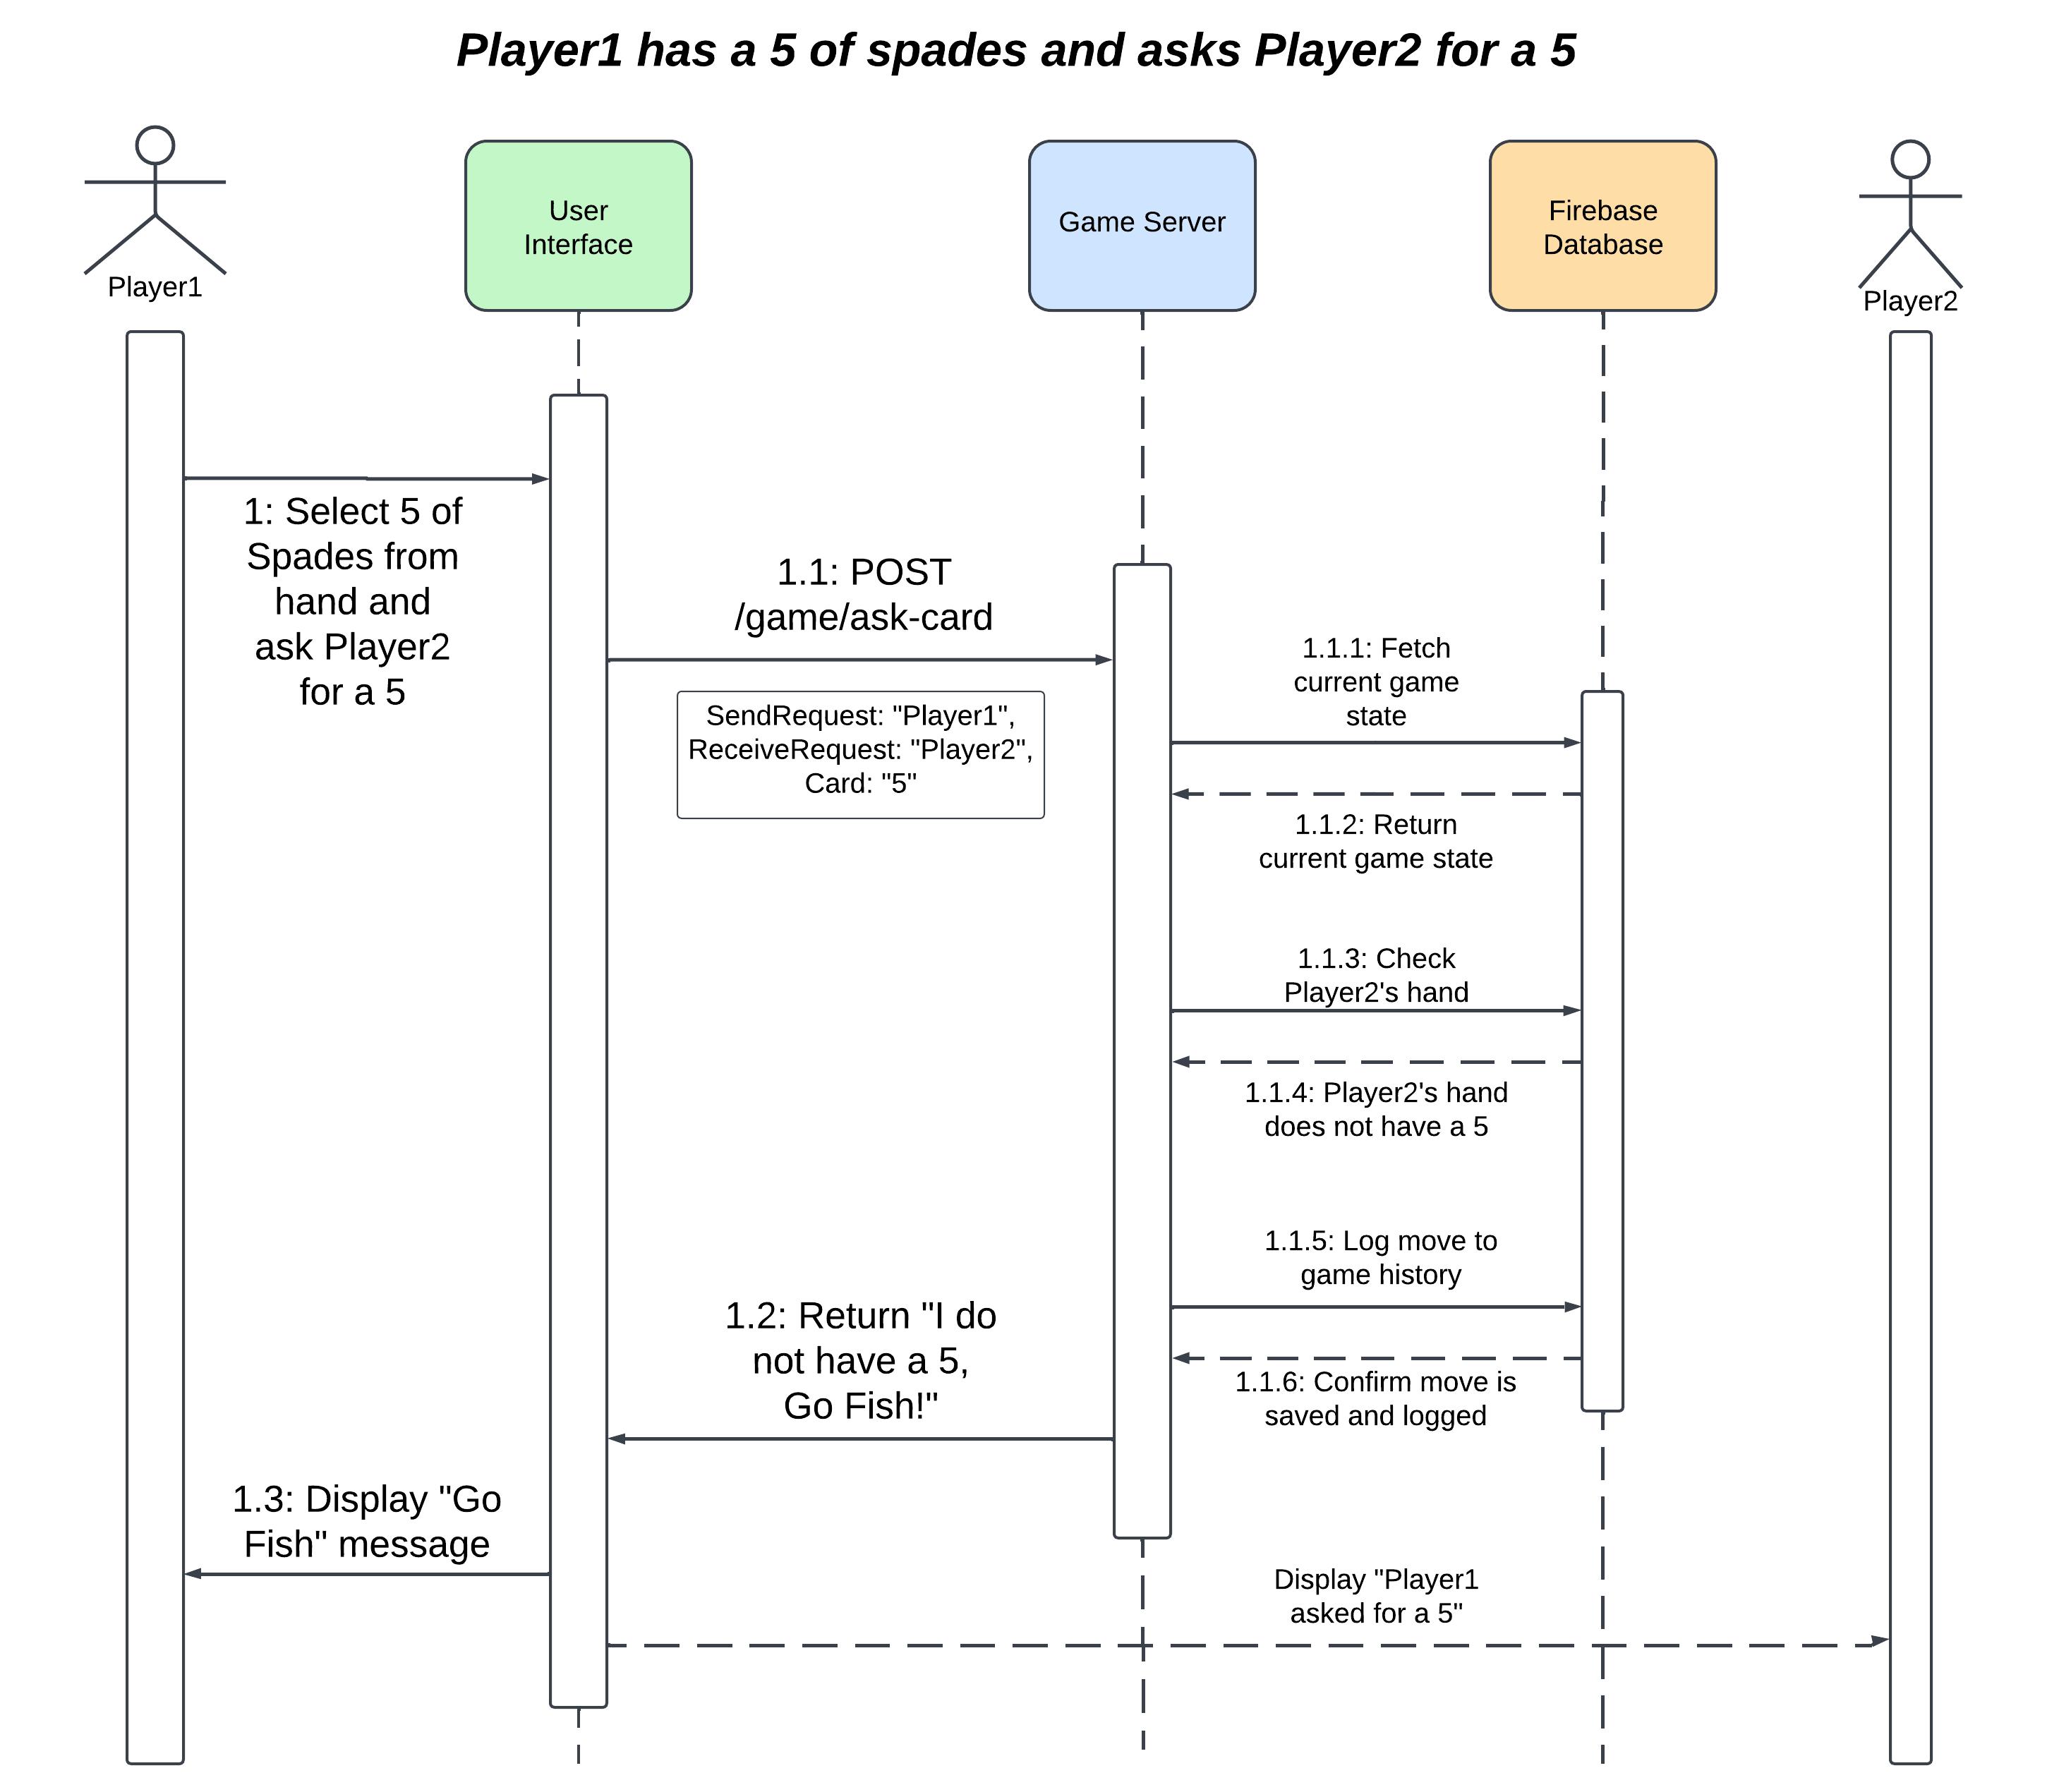
\includegraphics[width=1\linewidth]{CS482 Sequence Diagram Sprint 2.png}
    \caption{UML sequence diagram of Player1 asking Player2 for a card they do not have, resulting in Player1 being told to "Go Fish"}
    \label{fig:umlsequence}
\end{figure}

\noindent This UML sequence diagram illustrates the process of a player asking for a specific card during gameplay. In this scenario, Player1 selects a 5 of Spades from their hand and asks Player2 if they have any cards of the same rank. Player2, however, does not possess a 5, leading to the "Go Fish!" outcome for Player1.

\noindent The sequence begins with Player1 selecting the card and initiating a request through the game's user interface. This request is sent to the game server, which forwards it to the database to fetch Player2's current hand. The database responds with the data, enabling the server to check if Player2 has a 5. Upon finding that Player2 does not have the requested card, the server logs the move, saves the interaction in the game history, and returns a response to the user interface indicating that Player1 must "Go Fish!" The user interface then displays this message, completing the sequence.

\begin{figure}[htbp]
    \centering
    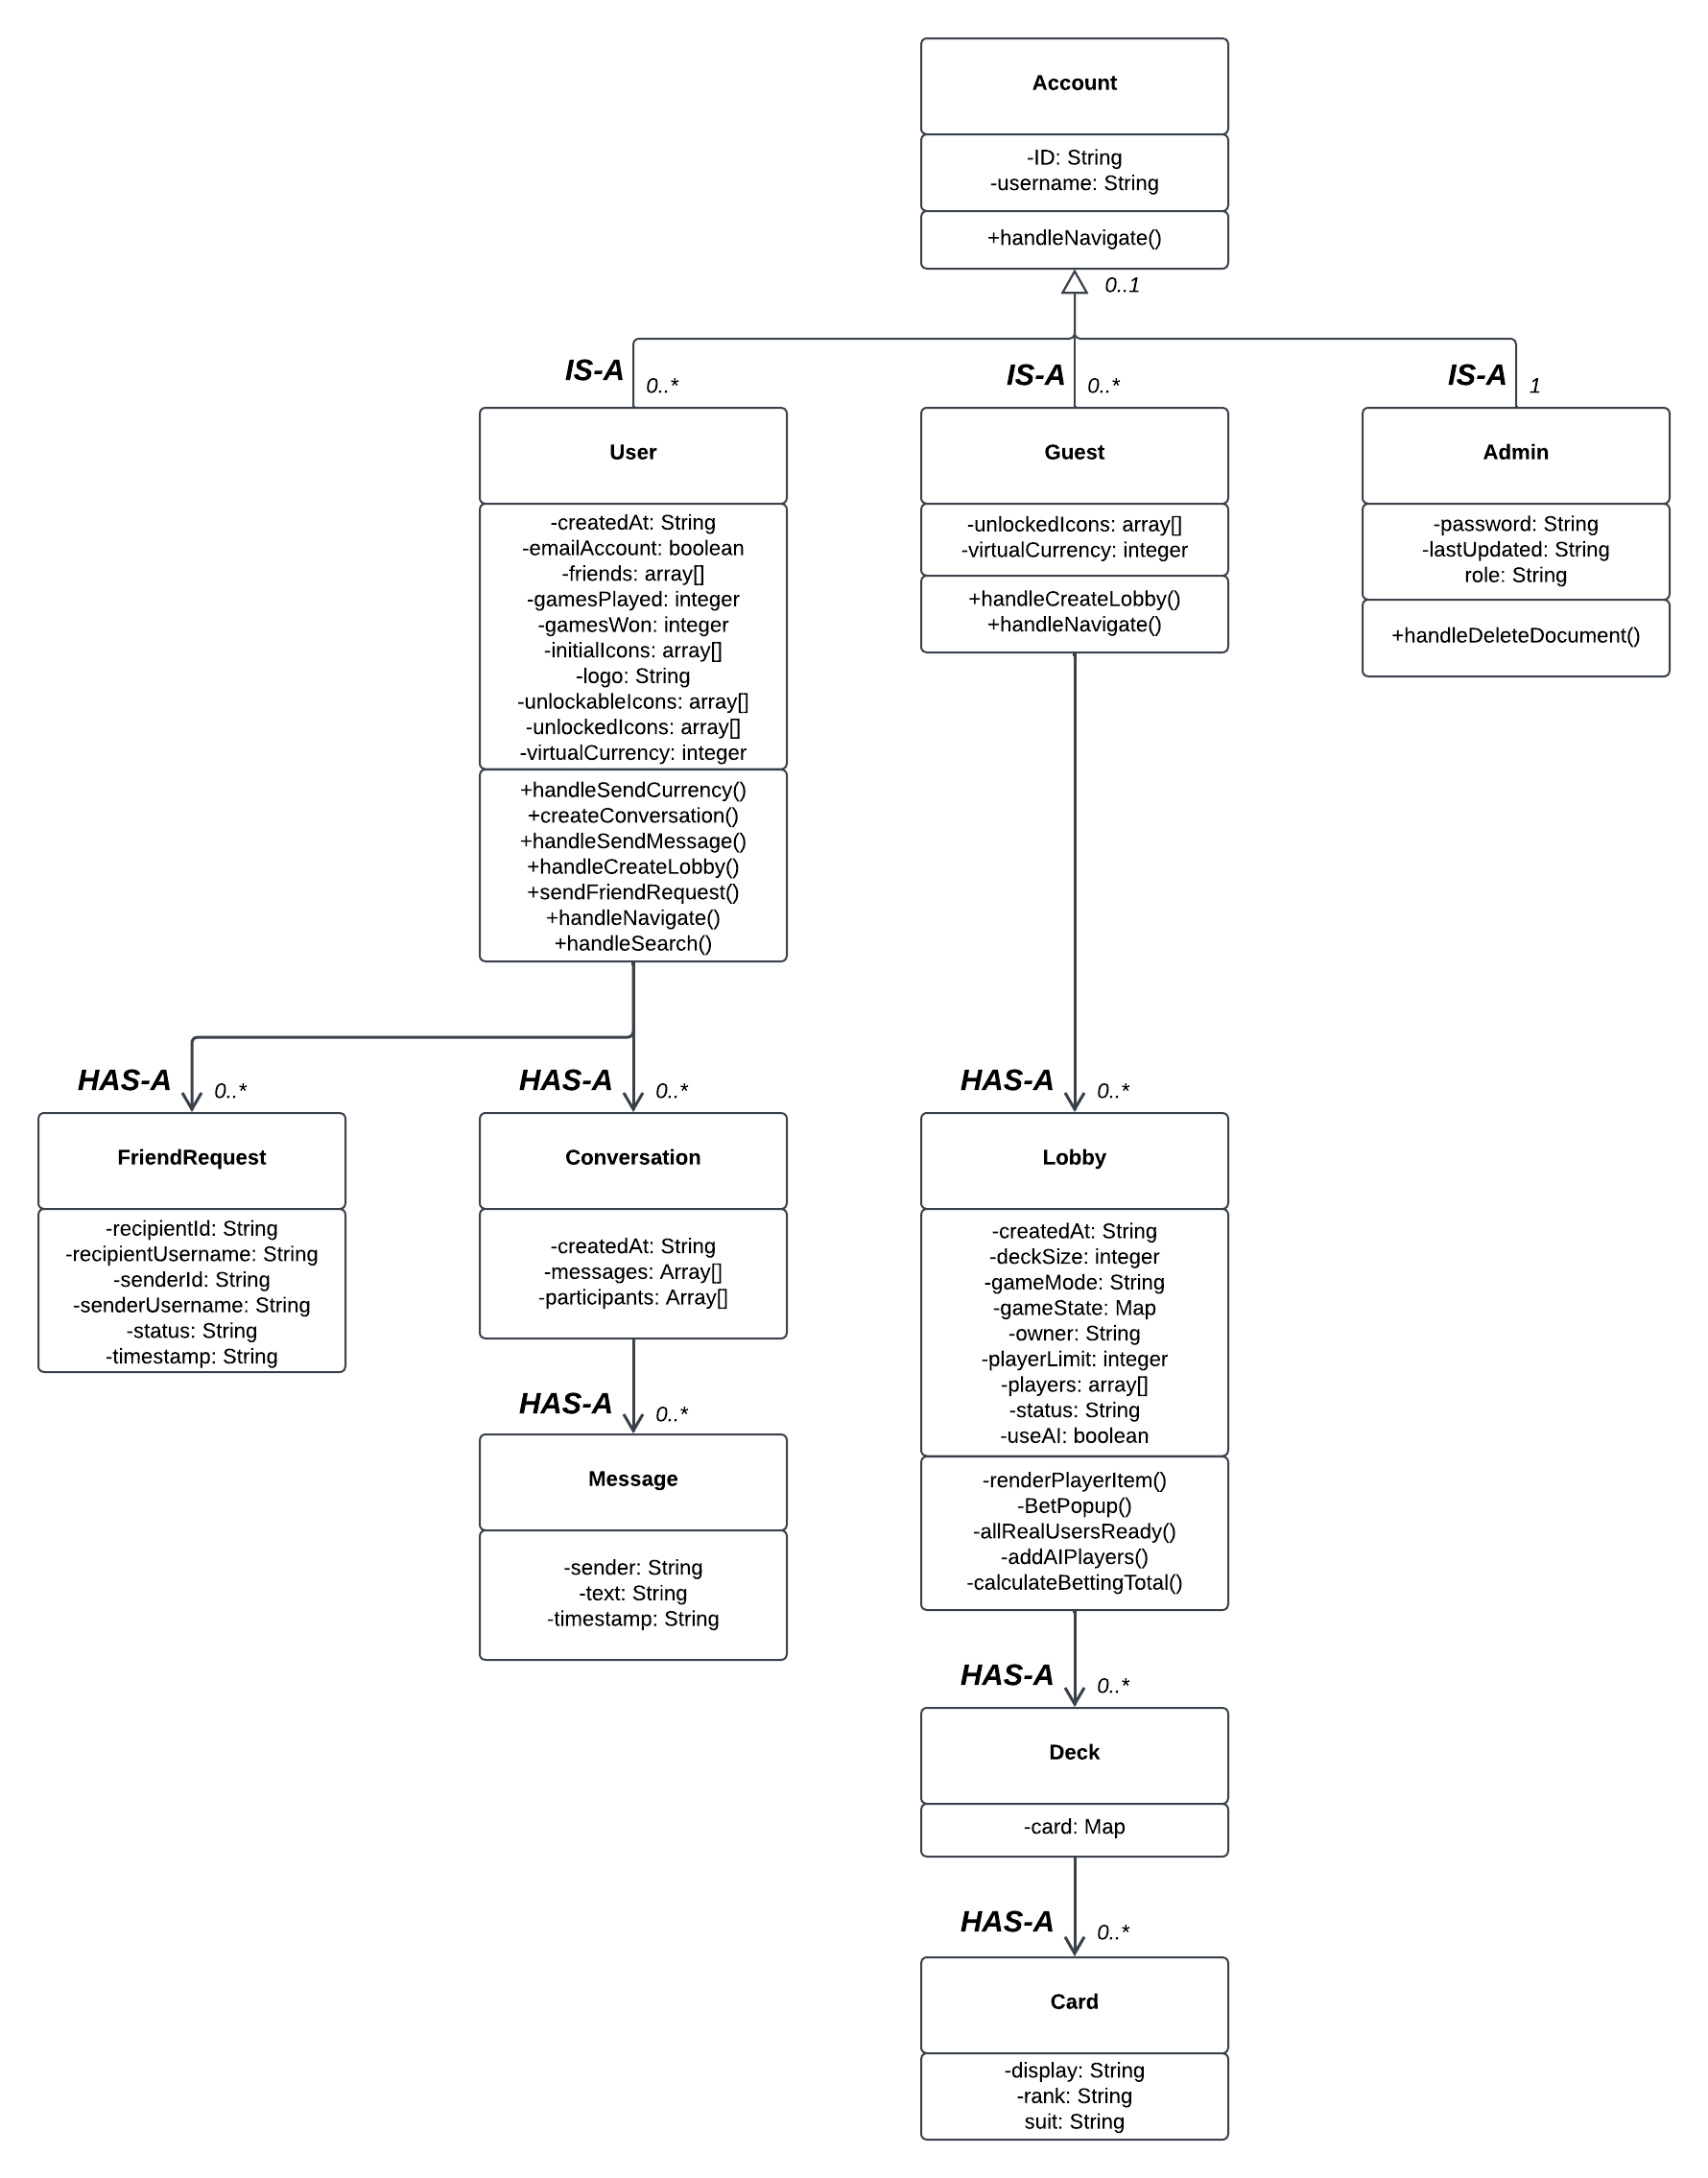
\includegraphics[width=1\linewidth]{CS482 Sequence Diagram Sprint 3.png}
    \caption{UML class diagram showing the system's structure, including key entities, their attributes, methods, and relationships.}
    \label{fig:umlclass}
\end{figure}

\noindent The UML class diagram outlines the system's architecture, showcasing the main classes, their attributes, methods, and relationships. At the top of the hierarchy is the Account class, which acts as the base class with attributes like ID and username and a method for navigation. Three subclasses inherit from Account: User, Guest, and Admin, each with distinct attributes and methods tailored to their specific roles.

\noindent The User class includes attributes such as friends, gamesPlayed, gamesWon, and virtualCurrency, along with methods for sending currency, creating conversations, and managing lobbies. The Guest class serves as a simplified version of the User, with limited attributes and methods focused on navigation and lobby creation. In contrast, the Admin class extends functionality by adding moderation capabilities, such as document deletion and role management.

\noindent The system’s functionality is built around several key components. The FriendRequest class handles friend requests, storing details such as the sender, recipient, and the status of the request. Messaging is managed by the Conversation class, which tracks participants and a collection of messages, with each message including information like the sender, text, and timestamp. The Lobby class oversees game lobbies, managing attributes such as the game mode, game state, and players, while also providing methods for player management, bet calculation, and AI control. Finally, the Deck and Card classes are responsible for managing the game’s deck and individual cards, with attributes defining their ranks, suits, and display properties.

\noindent The diagram highlights important relationships between components: IS-A relationships represent inheritance, while HAS-A relationships show composition or aggregation. It demonstrates how the components work together to support the system's functionality. The focus is on maintaining modularity and scalability, making it easier to expand or adapt the system in the future.

\pagebreak

\appendix
\clearpage 
\pagebreak
\section*{Appendix: Test Cases}
\addcontentsline{toc}{section}{Appendix: Test Cases}

\section{Test Cases}
We utilized Jest in conjunction with the React Testing Library in order to produce comprehensive test cases for our application. Our focus was on testing the main functionality of each component including form inputs, logo selection, page navigation, and many more.

\noindent

\textbf{Account Registration/Signing up}
\begin{itemize}
    \item Testcase 1: User doesn't input a username
    \begin{itemize}
        \item Input: Email and password filled out properly, but username field is left empty
        \item Expected Output: "Please enter your username"
    \end{itemize}

    \item Testcase 2: User inputs a username, but not a logo
    \begin{itemize}
        \item Input:
            \begin{itemize}
                \item Email: "kobe24"
                \item Password: ""
            \end{itemize}
        \item Expected Output: "Please choose an icon and enter a username"
    \end{itemize}

    \item Testcase 3: No Email and password
    \begin{itemize}
        \item Input: Email and password fields left empty
        \item Expected Output: "Please enter your email and password"
    \end{itemize}

    \item Testcase 4: Email with no '@' symbol
    \begin{itemize}
        \item Input:
            \begin{itemize}
                \item Email: "Spongebob"
                \item Password: "Squarepants"
            \end{itemize}
        \item Expected Output: "Invalid Email"
    \end{itemize}

    \item Testcase 5: Allows for selection of logo
    \begin{itemize}
        \item Input: User selects Dog icon for logo
        \item Expected Output: "logo: 'Dog'"
    \end{itemize}

    \item Testcase 6: Signing up using email and password
    \begin{itemize}
        \item Input: 
            \begin{itemize}
                \item Email: "spongebob@krustykrab.com"
                \item Password: "hello123"
                \item Username: "pattyflipper"
                \item Logo: "Bot"
            \end{itemize}
        \item Expected Output: "Account created"
    \end{itemize}

    \item Testcase 7: Signing up using Google
    \begin{itemize}
        \item Input: Gmail user information
        \item Expected Output: "Enter your username and select a logo"
    \end{itemize}

    \item Testcase 8: Returning to home during account registration process
    \begin{itemize}
        \item Input: Clicking the sign up button, then clicking the home button
        \item Expected Output: User is returned to opening page and no account is created
    \end{itemize}

    \item Testcase 9: Returns to previous page during process of signing up with an email and password
    \begin{itemize}
        \item Input: 
            \begin{itemize}
                \item Email: "test@testing.com"
                \item Password: "testtest"
                \item User then selects "Back" button
            \end{itemize}
        \item Expected Output: User is returned to sign-up page where they can choose to create an account with Google or using an email and password
    \end{itemize}
\end{itemize}

\noindent
\textbf{Logging into an Existing Account}
\begin{itemize}
    \item Testcase 1: No email or password is inputted
    \begin{itemize}
        \item Input: Leave email and password fields empty
        \item Expected Output: "Please enter email and password"
    \end{itemize}

    \item Testcase 2: Invalid email format
    \begin{itemize}
        \item Input: 
            \begin{itemize}
                \item Email: "InvalidEmail"
                \item Password: "password123"
            \end{itemize}
        \item Expected Output: "Please enter a valid email address"
    \end{itemize}

    \item Testcase 3: Password too short
    \begin{itemize}
        \item Input: 
            \begin{itemize}
                \item Email: "test@example.com"
                \item Password: "123"
            \end{itemize}
        \item Expected Output: "Password must be at least 6 characters"
    \end{itemize}

    \item Testcase 4: Successful login with valid credentials
    \begin{itemize}
        \item Input: 
            \begin{itemize}
                \item Email: "test@example.com"
                \item Password: "password123"
                \item Logo: "dog"
            \end{itemize}
        \item Expected Output: Logs user into their account and directs user to the home page where their information is displayed
    \end{itemize}

    \item Testcase 5: Invalid login credentials
    \begin{itemize}
        \item Input:
            \begin{itemize}
                \item Email: "test@example.com"
                \item Password: "wrongpassword"
            \end{itemize}
        \item Expected Output: "Invalid login credentials"
    \end{itemize}
\end{itemize}

\noindent
\textbf{Home Page/Main Menu}
\begin{itemize}
    \item Testcase 1: Loading guest user data
    \begin{itemize}
        \item Input: 
            \begin{itemize}
                \item Username = "testGuest"
                \item Logo = "dog"
            \end{itemize}
        \item Expected Output: 
            \begin{itemize}
                \item The username 'testGuest' is displayed and the dog icon is displayed as well
            \end{itemize}
    \end{itemize}
    
    \item Testcase 2: Load registered user data
    \begin{itemize}
        \item Input:
            \begin{itemize}
                \item item Username: "ExampleUser"
                \item Logo: "Cat"
                \item Virtual Currency: 1000
            \end{itemize}
        \item Expected Output: The username 'ExampleUser' is displayed, virtual currency is 1000, and the user logo of a cat is displayed
    \end{itemize}

    \item Testcase 3: Guest logout
    \begin{itemize}
        \item Input: Guest user logs out of home page
        \item Expected Output: The 'deleteDoc' function is called and the user is navigated to the '/' route.
    \end{itemize}
    
    \item Testcase 4: Navigation to different pages
    \begin{itemize}
        \item Input: Render the Home component
        \item Expected Output:
            \begin{itemize}
                \item Clicking the 'Friends' button navigates to the '/Friends' route
                \item Clicking the 'Messages' button navigates to the '/Messages' route
                \item Clicking the 'Shop' button navigates to the '/shop' route
            \end{itemize}
    \end{itemize}

    \item Testcase 5: Create Lobby dropdown
    \begin{itemize}
        \item Input: Render the Home component
        \item Expected Output: Clicking the 'Create Lobby' button displays the 'Public Lobby' and 'Private Lobby' options
    \end{itemize}
    
    \item Testcase 6: Join Lobby dropdown
    \begin{itemize}
        \item Input: Render the Home component
        \item Expected Output: Clicking the 'Join Lobby' button displays the 'Join Public' and 'Join Private' options
    \end{itemize}
    
    \item Testcase 7: Lobby owner left message display
    \begin{itemize}
        \item Input: Set 'ownerLeftMessage' in localStorage to 'The lobby owner has left'
        \item Expected Output: The message 'The lobby owner has left' is displayed and the 'ownerLeftMessage' key is removed from localStorage
    \end{itemize}
    
    \item Testcase 8: Admin support screen display toggled visible/invisible
    \begin{itemize}
        \item Input: Clicking on the "Admin Support" Button
        \item Expected Output: Initially, the admin support screen is not visible. Then, clicking the 'Admin Support' button opens the support modal. Clicking the 'Close' button in the support modal closes it
    \end{itemize}
    
    \item Testcase 9: Lobby dropdown closing on outside click
    \begin{itemize}
        \item Input: Clicking on "Create Lobby" button
        \item Expected Output: Clicking outside the dropdown (on the document body) closes the dropdown
    \end{itemize}
\end{itemize}

\noindent
\textbf{Joining a Public Lobby}
\begin{itemize}
    \item Testcase 1: Fetches and displays available lobbies
    \begin{itemize}
        \item Input:
            \begin{itemize}
                \item Lobby 1: Player username "Player1", logo "Cat", player limit 4, lobby type "public", use AI: true
                \item Lobby 2: Player username "Player2", logo "Dog", player limit 4, lobby type "public", use AI: false
            \end{itemize}
        \item Expected Output: The UI displays "Open Lobbies" and the player usernames "Player1" and "Player2".
    \end{itemize}

    \item Testcase 2: Navigates to the lobby page when Join Lobby is clicked
    \begin{itemize}
        \item Input:
            \begin{itemize}
                \item Lobby 1: Player username "Player1", logo "Cat", player limit 4, lobby type "public", use AI: true
            \end{itemize}
        \item Expected Output: The page navigates to the route "/lobby/1".
    \end{itemize}

    \item Testcase 3: Shows 'No lobbies available' message when no lobbies are available
    \begin{itemize}
        \item Input: Empty lobby list
        \item Expected Output: The UI displays "No lobbies available at the moment."
    \end{itemize}

    \item Testcase 4: Navigates back to the previous page when Back button is clicked
    \begin{itemize}
        \item Input: User clicks on the "Back" button
        \item Expected Output: The page navigates back to the previous route.
    \end{itemize}
\end{itemize}

\noindent
\textbf{Joining a Private Lobby}
\begin{itemize}
    \item Testcase 1: Renders the join private lobby form
    \begin{itemize}
        \item Input: Load the `JoinPrivate` component.
        \item Expected Output: The UI displays a form with the placeholder "Enter Lobby Code" and a button labeled "Join Lobby".
    \end{itemize}

    \item Testcase 2: Displays error if no lobby code is entered
    \begin{itemize}
        \item Input: User clicks on the "Join Lobby" button without entering any code.
        \item Expected Output: The UI displays "Please enter a lobby code."
    \end{itemize}

    \item Testcase 3: Displays error for invalid lobby code
    \begin{itemize}
        \item Input: User enters "INVALIDCODE" in the input field and clicks "Join Lobby".
        \item Expected Output: The UI displays "Invalid or inactive lobby code."
    \end{itemize}

    \item Testcase 4: Displays lobby details on valid lobby code
    \begin{itemize}
        \item Input:
            \begin{itemize}
                \item User enters "VALIDCODE" in the input field and clicks "Join Lobby".
                \item Mock lobby data with id "lobby123", player limit 10, use AI: true, and players "Player1" (logo: "Cat") and "Player2" (logo: "Dog").
            \end{itemize}
        \item Expected Output: The UI displays "Lobby Details" along with the player names "Player1" and "Player2".
    \end{itemize}

    \item Testcase 5: Resets to join form when Back button is clicked from lobby details view
    \begin{itemize}
        \item Input: User enters "VALIDCODE", clicks "Join Lobby", and then clicks the "Back" button from the lobby details view.
        \item Expected Output: The UI returns to the initial form with the placeholder "Enter Lobby Code".
    \end{itemize}

    \item Testcase 6: Navigates to lobby on Join Lobby button click
    \begin{itemize}
        \item Input:
            \begin{itemize}
                \item User enters "VALIDCODE", clicks "Join Lobby", and then clicks the "Join Lobby" button within the lobby details view.
                \item Mock lobby data with id "lobby123".
            \end{itemize}
        \item Expected Output: The page navigates to the route "/lobby/lobby123".
    \end{itemize}
\end{itemize}

\noindent
\textbf{Admin Support}
\begin{itemize}
    \item Testcase 1: Renders the support popup with form elements
    \begin{itemize}
        \item Input: Load the `Support` component.
        \item Expected Output: The UI displays a text area with the placeholder "What do you need help with?", and buttons labeled "Send" and "Close".
    \end{itemize}

    \item Testcase 2: Does not submit if message is empty
    \begin{itemize}
        \item Input: User clicks the "Send" button without entering any message.
        \item Expected Output: The `addDoc` function is not called.
    \end{itemize}

    \item Testcase 3: Submits a message and calls `onClose`
    \begin{itemize}
        \item Input: User enters "I need help!" in the input field and clicks the "Send" button and mock collection returns "mockCollection".
        \item Expected Output: 
            \begin{itemize}
                \item The `addDoc` function is called with the parameters: "mockCollection", a message object containing `userId: "test-user"`, `message: "I need help!"`, and a `timestamp`.
                \item The `onClose` function is called.
            \end{itemize}
    \end{itemize}

    \item Testcase 4: Logs an error if `addDoc` fails
    \begin{itemize}
        \item Input: User enters "Test error" in the input field and clicks the "Send" button.
        \item Expected Output: The console logs an error message "Error sending message: " followed by the error object.
    \end{itemize}

    \item Testcase 5: Calls `onClose` when Close button is clicked
    \begin{itemize}
        \item Input: User clicks the "Close" button. 
        \item Expected Output: The `onClose` function is called.
    \end{itemize}
\end{itemize}

\subsection{New Working Testcases}
For the following testcases they are all test-able and working.

\textbf{Sending Messages}
\begin{itemize}
    \item Testcase 1: User sends an empty message
    \begin{itemize}
        \item Input: Message = ""
        \item Expected Output: "Message cannot be empty"
    \end{itemize}

    \item Testcase 2: User sends a message to a valid conversation
    \begin{itemize}
        \item Input: Message = "Hello!" and existing conversation is selected
        \item Expected Output: Message successfully sent and appears in chat history
    \end{itemize}

    \item Testcase 3: User attempts to send a message without a selected conversation
    \begin{itemize}
        \item Input: Message = "Hello!" but no selected conversation
        \item Expected Output: "No conversation selected"
    \end{itemize}
\end{itemize}

\noindent
\textbf{Game Mechanics of Go Fish}
\begin{itemize}
    \item Testcase 1: Game setup with correct card distribution
    \begin{itemize}
        \item Input: Start a game with 4 players
        \item Expected Output: Each player is dealt 5 cards, and the remaining cards are placed in the middle of the table as the deck.
    \end{itemize}

    \item Testcase 2: Player asks another player for a card they have
    \begin{itemize}
        \item Input: Player A has 2 Aces and asks Player B for Aces (Player B has 1 Ace)
        \item Expected Output: Player B gives 1 Ace to Player A, resulting in Player A holding 3 Aces.
    \end{itemize}

    \item Testcase 3: Player asks another player for a card they don’t have
    \begin{itemize}
        \item Input: Player A asks Player C for Kings (Player C has no Kings)
        \item Expected Output: Player A draws a card from the deck. If it’s a King, Player A goes again. Otherwise, Player A's turn ends.
    \end{itemize}

    \item Testcase 4: Player completes a set
    \begin{itemize}
        \item Input: Player B collects all 4 Queens
        \item Expected Output: Player B places the set of 4 Queens face-up on the table.
    \end{itemize}

    \item Testcase 5: Player runs out of cards during their turn
    \begin{itemize}
        \item Input: Player A has 1 card, gives it away, leaving them with 0 cards
        \item Expected Output: Player A draws 5 new cards from the deck.
    \end{itemize}

    \item Testcase 6: Player draws the last card from the deck
    \begin{itemize}
        \item Input: Deck contains 1 remaining card, Player A goes fishing
        \item Expected Output: Player A draws the final card, deck is now empty.
    \end{itemize}

    \item Testcase 7: Game ends and calculates winner
    \begin{itemize}
        \item Input: All cards from the deck are used and players run out of cards
        \item Expected Output: Game ends, and the player with the most sets wins.
    \end{itemize}
\end{itemize}

\noindent
\textbf{Searching for Users to Message}
\begin{itemize}
    \item Testcase 1: User searches for a nonexistent username
    \begin{itemize}
        \item Input: Username = "NonexistentUser"
        \item Expected Output: "User not found"
    \end{itemize}

    \item Testcase 2: User searches for themselves (currently logged-in user)
    \begin{itemize}
        \item Input: Username = Current user’s username
        \item Expected Output: "You cannot search for yourself"
    \end{itemize}

    \item Testcase 3: User searches with an empty search field
    \begin{itemize}
        \item Input: Username = ""
        \item Expected Output: "Please enter a username to search"
    \end{itemize}

    \item Testcase 4: User searches for an existing username
    \begin{itemize}
        \item Input: Username = "existingUser"
        \item Expected Output: Display the user’s username and button to start a new conversation
    \end{itemize}
\end{itemize}

\noindent
\textbf{\textcolor{blue}{Shop Functionality Test Cases}}
\begin{itemize}
    \item Testcase 1: User tries to purchase an item they cannot afford
    \begin{itemize}
        \item Input: User currency = 100, Item price = 200
        \item Expected Output: "You need more money" error message, purchase unsuccessful
    \end{itemize}

    \item Testcase 2: User tries to purchase an item they already own
    \begin{itemize}
        \item Input: User inventory includes Item ID = 1 (Apple), User attempts to buy Item ID = 1 again
        \item Expected Output: "You already own this item" error message, purchase unsuccessful
    \end{itemize}

    \item Testcase 3: Guest user makes a valid purchase
    \begin{itemize}
        \item Input: User type = Guest, User currency = 500, Item price = 200, Item ID = 2 (Banana)
        \item Expected Output:
        \begin{itemize}
            \item User currency updated to 300
            \item Item added to inventory
            \item Success message: "You bought Banana!"
        \end{itemize}
    \end{itemize}

    \item Testcase 4: Logged-in user makes a valid purchase
    \begin{itemize}
        \item Input: User type = Logged-in user, User currency = 1000, Item price = 300, Item ID = 4 (Grape)
        \item Expected Output:
        \begin{itemize}
            \item User currency updated to 700
            \item Item added to inventory in Firestore
            \item Success message: "You bought Grape!"
        \end{itemize}
    \end{itemize}

    \item Testcase 5: User tries to purchase with no authentication (no user or guest)
    \begin{itemize}
        \item Input: No valid authentication, attempt to purchase Item ID = 5 (Candy)
        \item Expected Output: "Transaction failed: User does not exist" error message, purchase unsuccessful
    \end{itemize}

    \item Testcase 6: Background music toggles correctly
    \begin{itemize}
        \item Input: Toggle music button clicked when music is playing
        \item Expected Output: Music pauses, button text changes to "Music"
    \end{itemize}

    \item Testcase 7: User navigates back to home
    \begin{itemize}
        \item Input: Click "Home" button in the shop
        \item Expected Output: Music stops, user navigated to `/home`
    \end{itemize}

    \item Testcase 8: Shop items display correctly
    \begin{itemize}
        \item Input: Inventory includes Item ID = 3 (Cherry), User currency = 500
        \item Expected Output:
        \begin{itemize}
            \item All shop items displayed with correct name, price, and icon
            \item "Purchased" label visible for Item ID = 3, purchase button disabled for it
        \end{itemize}
    \end{itemize}

    \item Testcase 9: User data is correctly fetched on component mount
    \begin{itemize}
        \item Input: Logged-in user with 700 coins and inventory including Item ID = 6 (Pizza)
        \item Expected Output:
        \begin{itemize}
            \item User currency displayed as 700
            \item Inventory reflects ownership of Pizza, purchase button disabled for it
        \end{itemize}
    \end{itemize}
\end{itemize}
\pagebreak

\end{document}